\documentclass[11pt ,english,a4paper]{article}

\usepackage[english]{babel}
\usepackage[IL2]{fontenc}
\usepackage[utf8]{inputenc}
\usepackage{graphicx}
\usepackage{url}
\usepackage{hyperref}
\usepackage{times}
\usepackage{setspace}
\usepackage{float}
\usepackage{amsmath}

\setstretch{1.5}
\pagestyle{headings}

\title{Comparative Analysis of the Efficiency of Techniques for Detecting Misinformation in Healthcare Data\thanks{Semestral project in subject Engineering Methods, ac. year 2023/24, guidance: MSc. Mirwais Ahmadzai}}

\author{Alžbeta Žiarovská\\[2pt]
	{\small Slovak University of Technology in Bratislava}\\
	{\small Faculty of Informatics and Information Technologies}\\
	{\small \texttt{xziarovska@stuba.sk}}
	}

%ULOHA - zmenit na datum odovzdania
\date{\small 5th November 2023}



\begin{document}

\maketitle
\newpage

\begin{abstract}
This article offers a comparative analysis of efficiency of two machine learning techniques (Naïve Bayes and Support Vector Machine) used for information retrieval a detection of misinformation in a field of healthcare data. Article is a literature review and offers an outline of current situation of these machine learning methods. The comparison has found a negligible difference between the efficiency of the two compared techniques in data retrieval as means of combating medical misinformation by comparing metrics of accuracy, recall, precision and F1 score. There is a possibility of the use of my findings in everyday practice as these finding can point out that machine learning models are effective in sorting and retrieval of the medical information on the internet. 
\end{abstract}
\newpage

\section{Introduction}\label{intro}

It is known, that medical misinformation cause trouble \cite{wa19sys} and many researchers nowadays dive into the field of exploring possible use of machine learning techniques of misinformation detection in healthcare data \cite{bar21health}. Some of them summarize the information retrieval by these models whilst others try to create new techniques based on the existing ones, like Naïve Bayes and Support Vector Machine \cite{chap22unmask}.

\paragraph {Problem Definition} The great challenge in today's world of healthcare and medical information is the amount of the information available on the Internet. Even though it is useful to have easily accessible information, it also causes a problem. If the information is not understood correctly, it can increase fear and anxiety and ultimately lead to the delay of diagnosis and receiving the effective healthcare. \cite{wa19sys}. This issue became even more alarming after the global COVID-19 pandemic, where false medical information have created danger to public health or even lives \cite{war18dr}. 

\paragraph {Contribution} This article contributes to the already existing talk about fixing false health information. By reading and analyzing numerous studies, I was able to compare two machine learning techniques - Naïve Bayes and Support Vector Machine. This literature review does not only bring together ideas from various sources but as well attempts to make an introduction to how these models work in retrieving and detecting medical misinformation. The results I have found can be used by doctors and researchers, who are fighting the negative impact of misinformation in healthcare using machine learning techniques. 

\paragraph {} In this article I will talk about the big problem of false health information and how machine learning models Naïve Bayes and Support Vector Machine be used as a potential way of data retrieval that has ability to counter prevalence of misinformation in healthcare.

\section{Related work}

The topic of misinformation is quite often researched. Many of the works I came across use information retrieval done by machine learning as a way of recognizing misinformation found in healthcare data. Some of this work is focused on comparing the different machine learning techniques \cite{sha20mach}, \cite{pod19mach}. Focus of these researches are to introduce how these methods work. Other articles bring new way information retrieval technique \cite{chap22unmask} by combining the two, or even more techniques. Plenty of research have been also done in a field of processing medical misinformation, which is a important part of my article \cite{gu20misinfo}, \cite{cook15misinfo}, \cite{wa19sys}. These articles mostly focus on defining misinformation their possible cause and consequences. By making a revision of these works, I gain deeper knowledge of the healthcare misinformation and get a better starting point to make my own analysis.

\section{Methodology}\label{methodology}

For this article my methodology is based on an in-depth literature review of articles and researches debating medical misinformation and machine learning techniques used for information retrieval to detect such misinformation. Having a higher amount of the sources helped me  to understand a lot of different approaches to the same problem. 
The steps of my methodology were following:
\begin{enumerate}
\item{Finding various researches and studies debating the topic}
\item{Reading the sources and getting the knowledge of the problem}
\item{Extracting of relevant data from the literature}
\item{Concluding a comparison of efficiency of machine learning models}
\item{Analyzing the results and comparing the efficiency}
\end{enumerate}
 The two machine learning techniques I am focusing on are Naïve Bayes and Support Vector Machine. I introduce these techniques and compare their efficiency in order to establish which one is the most suitable for retrieving healthcare misinformation and its detection. The comparison of their efficiency is done by comparing the rates of accuracy, recall, precision and F1 score for detecting and correctly categorizing false information among true information. As I have used more articles and the numbers are varying a little in each of the sources, I have done a average of all the percentages of the efficiency given and established an estimate of which machine learning technique is more efficient by comparing the results.

\section{Misinformation in healthcare}\label{mih}

\paragraph{Difference between misinformation and disinformation}
The terms \emph{misinformation} and \emph{disinformation} are much the same, however, a small, but crucial difference can be distinguished. The difference between the two is a intention with which the false information is made accessible to the public and spread. Whilst the misinformation is usually created without direct intention of misleading and spreading false, meaning the person who put the information into the world might not actually know it is not true. On the other hand, disinformation is essentially created to spread false information. An example of such activity can be political propaganda \cite{gu20misinfo} \cite{cook15misinfo}. Even though the terms are not meaning the same, for the purpose of this article they are used as synonyms, because the author's knowledge, whether the information is factual, is negligible in the scope of its false recognition.

\paragraph{Historical development of concept of misinformation}%Lecture topic reaction
As the historical events have shown, the yearn for spreading not true information, either for amusement or with a goal of hurting someone, is old as a humanity itself \cite{bur17history}.

In the 16th century the writers have started to create completely false stories and plays in order to offer entertainment, but the drive was not only positive. During the French Revolution a rumor (in France called \emph{canard}) was used to discredit the queen Marie Antoinette, which doubtlessly did not help her in the later events of the French Revolution. \cite{bur17history} 

When the mass media took their place, the misleading was often used in order to change the opinion of the public during the times of war. For example during the World War II the Nazi propaganda was reaching the peaks of political propaganda ever. \cite{pos18short}

The rise of the \emph{hoax} in the era of the Internet is enormous and numerous fake websites were created.\cite{bur17history} Nowadays the information revolution by the Internet has brought many ways of spreading false information, but the way of their detection is not yet perfectly defined and therefore there is need for effective adaptive mechanisms.

\paragraph{Health care misinformation}
A vast majority of people is using the Internet and social media for entertainment or information seeking. However, with the possibility of immediate communication and sharing, it has become easy to spread misinformation online \cite{wa19sys}. During the COVID-19 pandemic there have been a great amount of healthcare misinformation spread regarding vaccines and their effectiveness \cite{chap22unmask}. Internet is easily accessible and more and more people are looking for relevant health information without the proper knowledge of how to distinguish, whether the information is true. This can lead to unintentionally getting false information, as many websites do not provide accurate medical information \cite{cook15misinfo}. Another example of current situation can be the popular misinformation about vaccines causing autism, which was repeatedly proven as nonfactual information \cite{wa19sys}. 
The spread of medical misinformation is not only occurring in the 21st century. In the past there was false information about public health impact of smoking spread by tobacco companies, which was later proven as false. \cite{cook15misinfo}.

\section{Machine learning techniques} \label{tech}

\paragraph{Societal context}%Lecture topic reaction
It is important to look out for the misinformation in everyday life.
I offer a list of some of the basic points that can help to recognize possible misinformation as effective and quick as possible in case there's immediate access to some of the machine learning techniques mentioned later in this Section: 
\begin{enumerate}
\item{\emph{Context}} - It is crucial to distinguish, whether the information is meant to be served as a fact to provide information or even to convince, or whether it is supposed to be taken as an exaggeration or sarcasm \cite{alh18fact}.
\item {\emph{Sentimental value}} - The goal of misinformation is often to scare people and spread panic. The difference between ratio of positive and negative in true and false claims is notable. Whilst in true claims the ratio is 71\% of positive words to 29\% of negative words, in misinformation sources this ratio is shifted the other way around with only 38\% of positive words and 62\% of negative words \cite{bar21health}.
\item {\emph{Sources}} - Perhaps the most important step might be to check the original sources of the claim \cite{gra17fact}. We need to look for the trustworthiness of the website or references, where did the author get the information from.
\end{enumerate}

\paragraph{Technology and people}%Lecture topic reaction
Besides using the tips for retrieving information on our own there were created websites that offer the result of the misinformation detection and can offer highly reliable picture of whether the checked claim is true or false. Using these websites can speed up the whole process and save the time needed for processing the information manually. These websites usually use the machine learning techniques explained in this Section. A few examples of such websites can be \emph{fullfact.org} or \emph{politifact.com} \cite{alh18fact}.

\subsection{Naïve Bayes}\label{nb}
The Naïve Bayes method is a linear probabilistic machine learning technique based on Bayes theorem. The method is based on comparing the possible misinformation and comparing it with the data-set previously used. This method uses probability of the events without taking their relation into the consideration, meaning, order of the words does not play role in the result. \cite{sha20mach}. This approach might not look to be the best, as the words have their order and are related one to other in articles. However, the opposite is true, as the linear models are capable of achieving high efficiency despite their simplicity \cite{pod19mach}. The accuracy of Naïve Bayes (as well as other machine learning methods) is also depended from which type of measuring the importance of the words in the documents is used. For the Naïve Bayes the results vary for all metrics (accuracy, recall, precision and F1 score). The closer analysis of  differences between the metrics and their comparison is given in Section \ref{analysis}. In the table \ref{table:nb} are mentioned the lowest and the highest percentages of each metrics according to sources used in this article. All of the percentages used can be found in Table \ref{table:results} in Section \ref{analysis}.

\begin{table}[H]
\centering
\begin{tabular}{|ll|ll|}
\hline
\multicolumn{2}{|l|}{Accuracy}           & \multicolumn{2}{l|}{Recall}      \\ \hline
\multicolumn{1}{|l|}{84.056\%\cite{sha20mach}} & 98.71\%\cite{bar21health} & \multicolumn{1}{l|}{70.53\%\cite{sha20mach}} & 98.70\%\cite{bar21health} \\ \hline
\multicolumn{2}{|l|}{Precision}      & \multicolumn{2}{l|}{F1 score}          \\ \hline
\multicolumn{1}{|l|}{84\%\cite{chap22unmask}} & 99.56\%\cite{bar21health} & \multicolumn{1}{l|}{81.67\%\cite{sha20mach}} & 99.13\%\cite{bar21health} \\ \hline
\end{tabular}
\caption{\centering Range of the results for Naïve Bayes according to multiple sources.}
\label{table:nb}
\end{table}


Formula for Naïve Bayes calculation: \cite{sha20mach}

\begin{equation}
P(A|B) = \frac{P(B|A)P(A)}{P(B)}
\end{equation}

\begin{itemize}
\item \emph{P(A\textbar B)} is the probability of event A happening supposing, that event B has already occurred \cite{jo03bayes}
\item \emph{P(B\textbar A)} is representing how possible the event B is, assuming that the event A is true \cite{jo03bayes}
\item \emph{P(A)} is the main event for which the probability of happening is calculated \cite{jo03bayes}
\item \emph{P(B)} is an event, which serves as an evidence based on the given data set and training results \cite{jo03bayes}
\end{itemize}

\subsection{Support Vector Machine}\label{svm}
Support vector machine might be classified as a binary technique, as its methodology is to divide the data it was given into two categories \cite{pod19mach} (in the case of misinformation detection into true and false information). The division is made by creating a hyperplane (a object in the vector space with one dimension less than the vector space itself). The objective is to identify the hyperplane with the greatest margin, the space between the hyperplane and the nearest data points in each category. After finding the hyperplane, analyzed data can be categorized based on its position relative to the hyperplane \cite{sha20mach}.
As it was mentioned in the section \ref{nb} about Naïve Bayes, the result can vary according to the technique used for analysis of the given data and for the Support Vector Machine the lowest and the highest percentages of each metrics can be found in Table \ref{table:svm}. As mentioned in Section \ref{nb}, the whole variety of results can be seen in Table \ref{table:results} in Section \ref{analysis}.

\begin{table}[H]
\centering
\begin{tabular}{|ll|ll|}
\hline
\multicolumn{2}{|l|}{Accuracy}           & \multicolumn{2}{l|}{Recall}      \\ \hline
\multicolumn{1}{|l|}{83\%\cite{chap22unmask}} & 95.05\%\cite{sha20mach} & \multicolumn{1}{l|}{84\%\cite{chap22unmask}} & 93.73\%\cite{sha20mach} \\ \hline
\multicolumn{2}{|l|}{Precision}      & \multicolumn{2}{l|}{F1 score}          \\ \hline
\multicolumn{1}{|l|}{85\%\cite{chap22unmask}} & 99.31\%\cite{bar21health} & \multicolumn{1}{l|}{84\%\cite{chap22unmask}} & 95.98\%\cite{bar21health} \\ \hline
\end{tabular}
\caption{\centering Range of the results for Support Vector Machine according to multiple sources.}
\label{table:svm}
\end{table}

\paragraph{Ethics and sustainability}%Lecture topic reaction
As I have established before, spread of false information in medical field can have risky and potentially fatal consequences. Therefore, the retrieval and detection of healthcare misinformation is significant. The machine learning techniques I have mentioned - Naïve Bayes and Support Vector Machine can be used for such purpose. \cite{chap22unmask}. Nevertheless, the incorporation of machine learning techniques requires careful approach, considering, that the data-sets used for training can be biased and generate inaccurate information. \cite{who21ethics}. Therefore there is a need to check, whether the data-sets are representing the population correctly, with adequate diversity. \cite{sch23aut}.

\section{Results and Analysis}\label{analysis}
In this section I compare their results and analyze their performance. To do so, I have searched of numeric expression of their efficiency in percentage. I used accuracy, recall, precision and F1 score to compare their efficiency. To correctly understand the equations for the metrics I have to explain some terms:

\begin{itemize}
\item \emph{True Positives} - amount of the claim correctly categorized as true
\item \emph{False Positives} - amount of the claim incorrectly categorized as true
\item \emph{True Negatives} - amount of the claim correctly categorized as false
\item \emph{False Negatives} - amount of the claim incorrectly categorized as false
\end{itemize}

\paragraph{} \emph{Accuracy} represents the correctness of categorizing health information as true or false. This number is calculated by dividing the correct categorizations and the total number of categorizations made. Accuracy is an efficient metric when the categories are distributed equally, as it might me misleading when one class is rarer than the other one \cite{aph18detect}. Equation for calculating accuracy \cite{sha20mach}:

\begin{equation}
Accuracy = \frac{\text{\emph{Correctly categorized data}}}{\text{\emph{Total number of categorizations}}}
\end{equation}

\emph{Precision} is the proportion of correctly identified medical misinformation among all the cases, which were classified as misinformation. Precision is preferably when the elimination of false positives is required \cite{aph18detect}. Equation for calculating precision \cite{sha20mach}:

\begin{equation}
Precision = \frac{True Positives}{True Positives + False Positives}
\end{equation}

\emph{Recall} introduces the proportion of accurately established health misinformation among all actual cases of misinformation. Recall is useful in situations, when false negatives are a big concern and the capture of the maximum amount of misinformation is needed \cite{aph18detect}. Equation for calculating recall \cite{sha20mach}:

\begin{equation}
Recall = \frac{True Positives}{True Positives + False Negatives}
\end{equation}

\emph{F1 Score} represents the harmonic average of precision and recall, which offers an equitable evaluation of the two. It is applicable when an uneven class distribution occurs \cite{aph18detect}. Equation for calculating f1 score \cite{sha20mach}:

\begin{equation}
F1 Score = \frac{2*Precision*Recall}{Precision + Recall}
\end{equation}

\paragraph{} As mentioned in Section \ref{methodology}, this analysis is based on review of existing literature, which allows me to access finding from multiple sources. Each source provides different results which can be found in Table \ref{table:results} with corresponding superscripts of the source that the number comes from. 

\begin{table}[H]
\centering
\begin{tabular}{lllll}
\cline{2-5}
                       & \multicolumn{4}{|l|}{Accuracy}  \\ [0.5ex]
\hline\hline
\multicolumn{1}{|l|}{Naive Bayes} & \multicolumn{1}{l|}{$88.37\%^{1}$} & \multicolumn{1}{l|}{$98.71\%^{2}$} & \multicolumn{1}{l|}{$85.85\%^{3}$} & \multicolumn{1}{l|}{ $84.06\%^{4}$}\\
\hline
\multicolumn{1}{|l|}{Support Vector Machine}& \multicolumn{1}{l|}{$84\%^{1}$} & \multicolumn{1}{l|}{$94.17\%^{2}$} & \multicolumn{1}{l|}{$90.95\%^{3}$} & \multicolumn{1}{l|}{$95.05\%^{4}$} \\ [1ex]
\hline\hline
\cline{2-5}
                       & \multicolumn{4}{|l|}{Recall}  \\ [0.5ex]
\hline\hline
\multicolumn{1}{|l|}{Naïve Bayes} & \multicolumn{1}{l|}{$84\%^{1}$} & \multicolumn{1}{l|}{$98.70\%^{2}$} & \multicolumn{1}{l|}{$-\%^{3}$} & \multicolumn{1}{l|}{ $70.53\%^{4}$}\\
\hline
\multicolumn{1}{|l|}{Support Vector Machine}& \multicolumn{1}{l|}{$84\%^{1}$} & \multicolumn{1}{l|}{$92.87\%^{2}$} & \multicolumn{1}{l|}{$-\%^{3}$} & \multicolumn{1}{l|}{$93.73\%^{4}$} \\ [1ex]
\hline\hline
\cline{2-5}
                       & \multicolumn{4}{|l|}{Precision}  \\ [0.5ex]
\hline\hline
\multicolumn{1}{|l|}{Naïve Bayes} & \multicolumn{1}{l|}{$84\%^{1}$} & \multicolumn{1}{l|}{$99.56\%^{2}$} & \multicolumn{1}{l|}{$-\%^{3}$} & \multicolumn{1}{l|}{ $96.98\%^{4}$}\\
\hline
\multicolumn{1}{|l|}{Support Vector Machine}& \multicolumn{1}{l|}{$85\%^{1}$} & \multicolumn{1}{l|}{$99.31\%^{2}$} & \multicolumn{1}{l|}{$-\%^{3}$} & \multicolumn{1}{l|}{$92.56\%^{4}$} \\ [1ex]
\hline\hline
\cline{2-5}
                       & \multicolumn{4}{|l|}{F1 score}  \\ [0.5ex]
\hline\hline
\multicolumn{1}{|l|}{Naïve Bayes} & \multicolumn{1}{l|}{$83.5\%^{1}$} & \multicolumn{1}{l|}{$99.13\%^{2}$} & \multicolumn{1}{l|}{$-\%^{3}$} & \multicolumn{1}{l|}{ $81.67\%^{4}$}\\
\hline
\multicolumn{1}{|l|}{Support Vector Machine}& \multicolumn{1}{l|}{$84\%^{1}$} & \multicolumn{1}{l|}{$95.98\%^{2}$} & \multicolumn{1}{l|}{$-\%^{3}$} & \multicolumn{1}{l|}{$93.14\%^{4}$} \\ [1ex]
\hline\hline
\end{tabular}
\caption{\centering Efficiency metrics (accuracy, recall, precision, F1 score) of machine learning techniques in misinformation detection according to various researches, 1 - \cite{chap22unmask}, 2 - \cite{bar21health}, 3 - \cite{pod19mach}, 4 - \cite{sha20mach}}
\label{table:results}
\end{table}

According to the results of this comparison, Support Vector Machine is slightly more efficient in processing medical misinformation with average percentage of success higher in accuracy (91.04\%), recall (90.2\%) and F1 score (91.04\%). However, the Naïve Bayes method is behind just by a little bit with the average percentage of accuracy (89.25\%), recall (84.41\%) and F1 score (88.1\%). In the terms of precision, Naïve Bayes has achieved higher percentage rate of 93.51\% compared to Support Vector Machine with 92.29\%. The average efficiency rate of information retrieval using Naïve Bayes or Support Vector Machine can be seen in Figure \ref{f:average}. This graph was created by making a harmonic average of all the results mentioned in Table \ref{table:results} for each metrics for both Naïve Bayes and Support Vector Machine.

\begin{figure}[H]
\centering
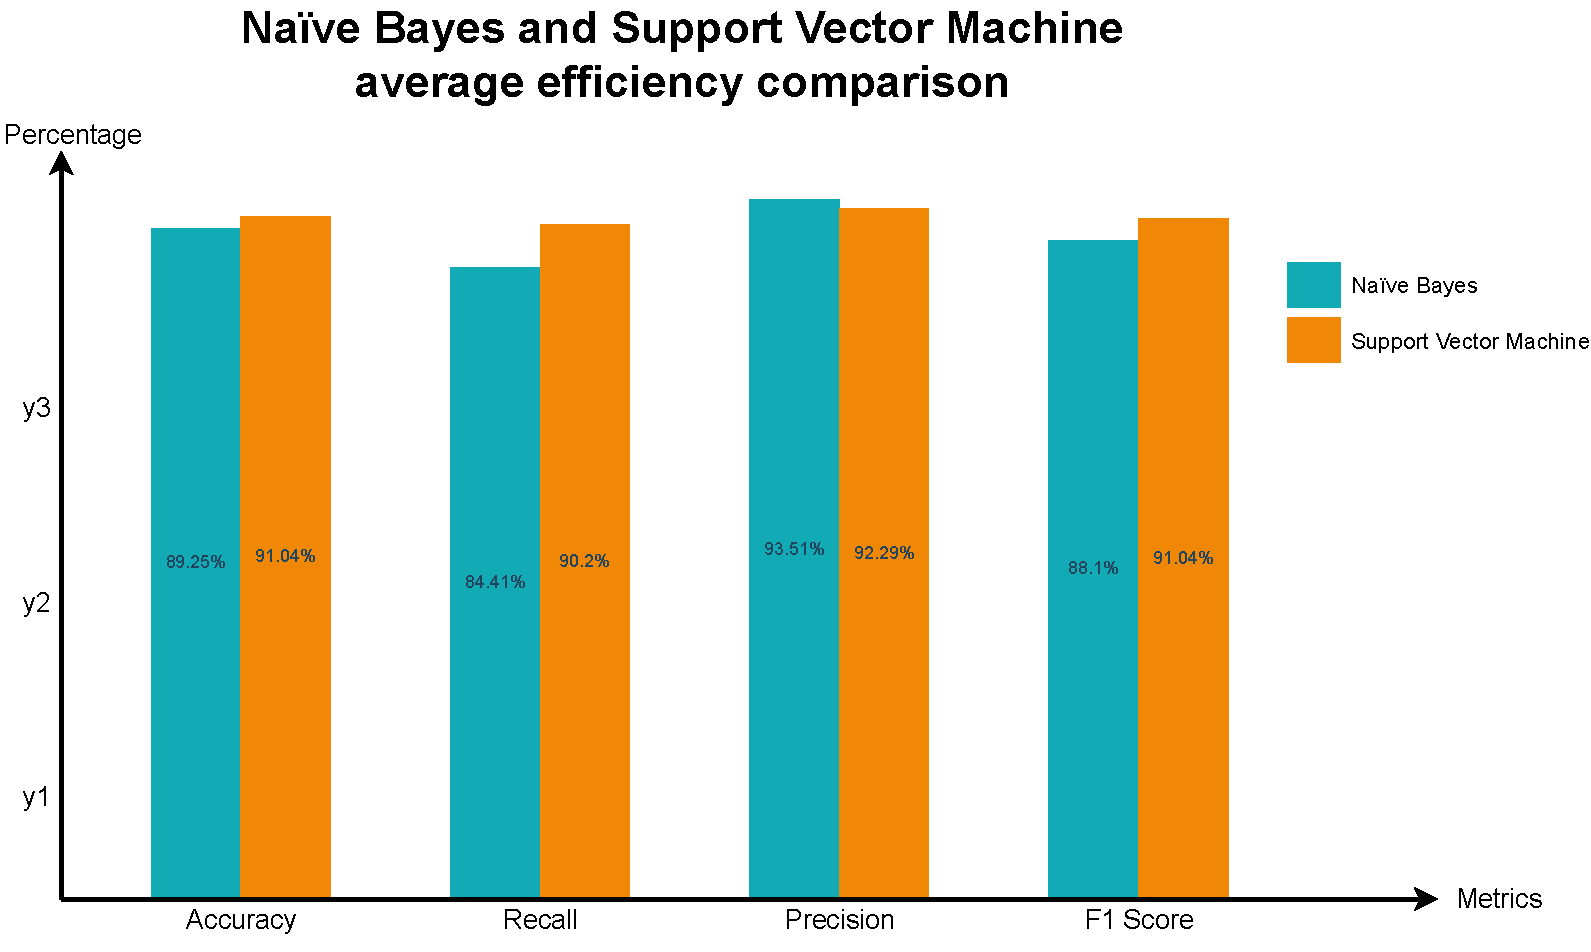
\includegraphics[scale=0.5]{average.pdf}
\caption{\centering Comparison of average values of each efficiency metric.}
\label{f:average}
\end{figure}

As pictured in Table \ref{f:average}, Support Vector Machine achieves higher success rate in accuracy, recall and F1 score. Naïve Bayes has a higher precision rate with 93.51\%. This can be a helpful information when choosing which one of them to apply. Recall is about not missing any misinformation among all the data-set, whilst precision is about only giving misinformation category to actual misinformation (being more precise), even for the toll of possibly not categorizing as much claims as recall. Precision has generally a lower number of false positives. 

\section{Discussion}

I have found several evidence to confirm, that machine learning techniques can be a very useful (and accurate) tool in retrieving and recognizing misinformation in healthcare with both Naïve Bayes and Support Vector Machine showing satisfactory performance. In my article I used percentages of accuracy, recall, precision and F1 score of these two machine learning techniques used for misinformation detection to analyze and compare their efficiency. 
The Support Vector Machine achieves a slightly higher accuracy, offering an overall higher correctness to some point. In the terms of precision and recall, Naïve Bayes shows higher precision, which might indicate it is able to identify medical misinformation with greater accuracy among the cases categorized as false information. 

This can be useful in cases, where the misinformation is threatening a human's life by any chance and there is an actual need of correctly marking the misinformation and only misinformation. However, precision can possibly categorize less claims compared to recall.

On the contrary, Support Vector Machine achieves a higher recall percentage, suggesting the fitter ability of identifying actual medical misinformation. The last metrics used was F1 Score. Giving the average of both precision and recall (f1 score), Support Vector Machine achieves a slightly better result.
Which one is chosen to retrieve the data might depend on context of the situation in which the technique is used. The Support Vector Machine is according to the result more efficient, however the difference is trivial. Naïve Bayes might have an advantage when looking for more precisely categorized medical misinformation. The results are not so greatly differing from each other and it shows, that machine learning techniques nowadays are highly advanced and can achieve significant results. The insignificant differences in the results also show the necessity of comparing multiple metrics to complexly evaluate their efficiency in recognizing the healthcare misinformation.
It is important to acknowledge, that my article is based on literature review of existing researches, which creates limitations by the range of the researches used for the purpose of this article.

\section{Conclusion}\label{conclusion}

This article is an in-depth literature review of articles researching misinformation retrieval and detection in healthcare data using machine learning methods. I have compared results from several resources and based on these I have created an analysis of two machine learning techniques I focused on. In order to provide analysis of their efficiency I came to conclusion, that the machine learning techniques are highly advanced and can efficiently differentiate between factual and nonfactual information. This can provide solution to the main problem I mentioned in the beginning of the article - people possibly not perceiving the information found on the Internet correctly. With the use of machine learning techniques there is a possibility of decreasing spread of medical misinformation by having effective tool for information processing.

\paragraph{Future Work} The work I have done and the results I have analyzed and compared might help to establish the use of machine learning techniques used of retrieving and detecting healthcare misinformation. Nonetheless, the evaluation of the results on real world data-sets using the same metrics and machine learning techniques is essential and would help to validate my findings. 

\newpage
\bibliography{127323_bibliography}
\bibliographystyle{unsrt}
\end{document}
